The best-fit BPL model of CR proton from this work are consistent with direct
measurements as shown in figure~\ref{fig:proton-flux}.
% The result also put weight on the previous study that we could take a
% benefit of brightness $\gamma$-ray from Earth's high atmosphere to indirectly observe cosmic
% ray spectrum which cause it’s luminosity.
We will need to determine whether the BPL model fits the data significantly better
than the SPL model does using likelihood ratio test to quantify the level of
confidence. We also plan to determine the statistical and total uncertainties of
the fit results by performing Monte Carlo simulations.
This work emphasizes that we could utilize the bright $\gamma$-ray emission
of the Earth's upper atmosphere to indirectly observe various properties of CRs.

\begin{figure}
    \centering
    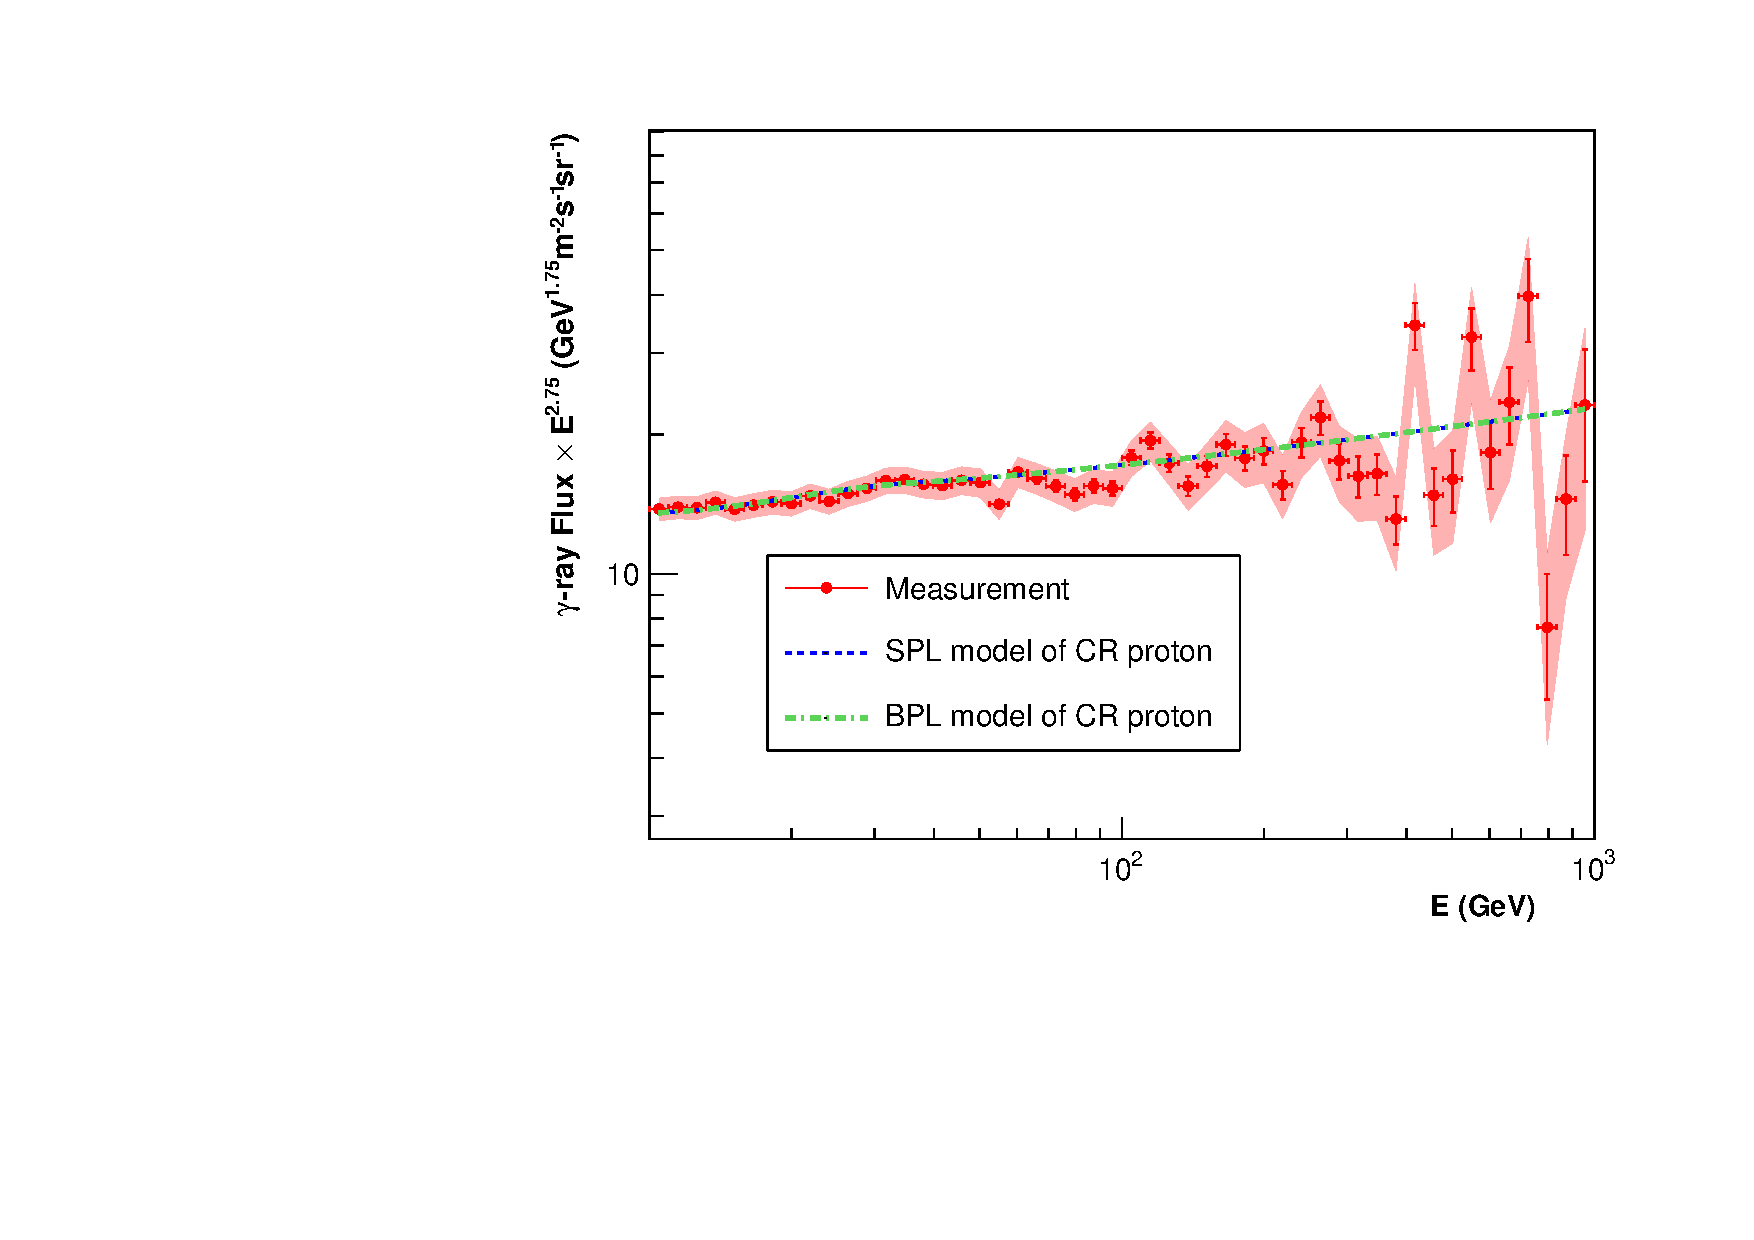
\includegraphics[width=0.8\textwidth]{img/fitted_result}
    % \caption{Measured $\gamma$-ray flux and the product from incident CRs}
    \caption{
        The $\gamma$-ray spectra calculated from the SPL (blue)
        and BPL (green) models of CR proton which best fit with the measured Earth's
        $\gamma$-ray spectrum in the thin-target regime (red).
    }
    \label{fig:gamma-flux}
\end{figure}


\begin{center}
\begin{table}
\centering
\caption{Best-fit CR proton spectral parameters.} 
\label{tb:bestparams}
\begin{tabular}{@{}l*{15}{l}}
\br
CR proton model&Index 1&Index 2&$E_\text{break}$ (GeV)\\
\mr
SPL&2.70&-&-\\
BPL&2.86&2.63&333\\
\br
\end{tabular}
\end{table}
\end{center}


\begin{figure}
    \centering
    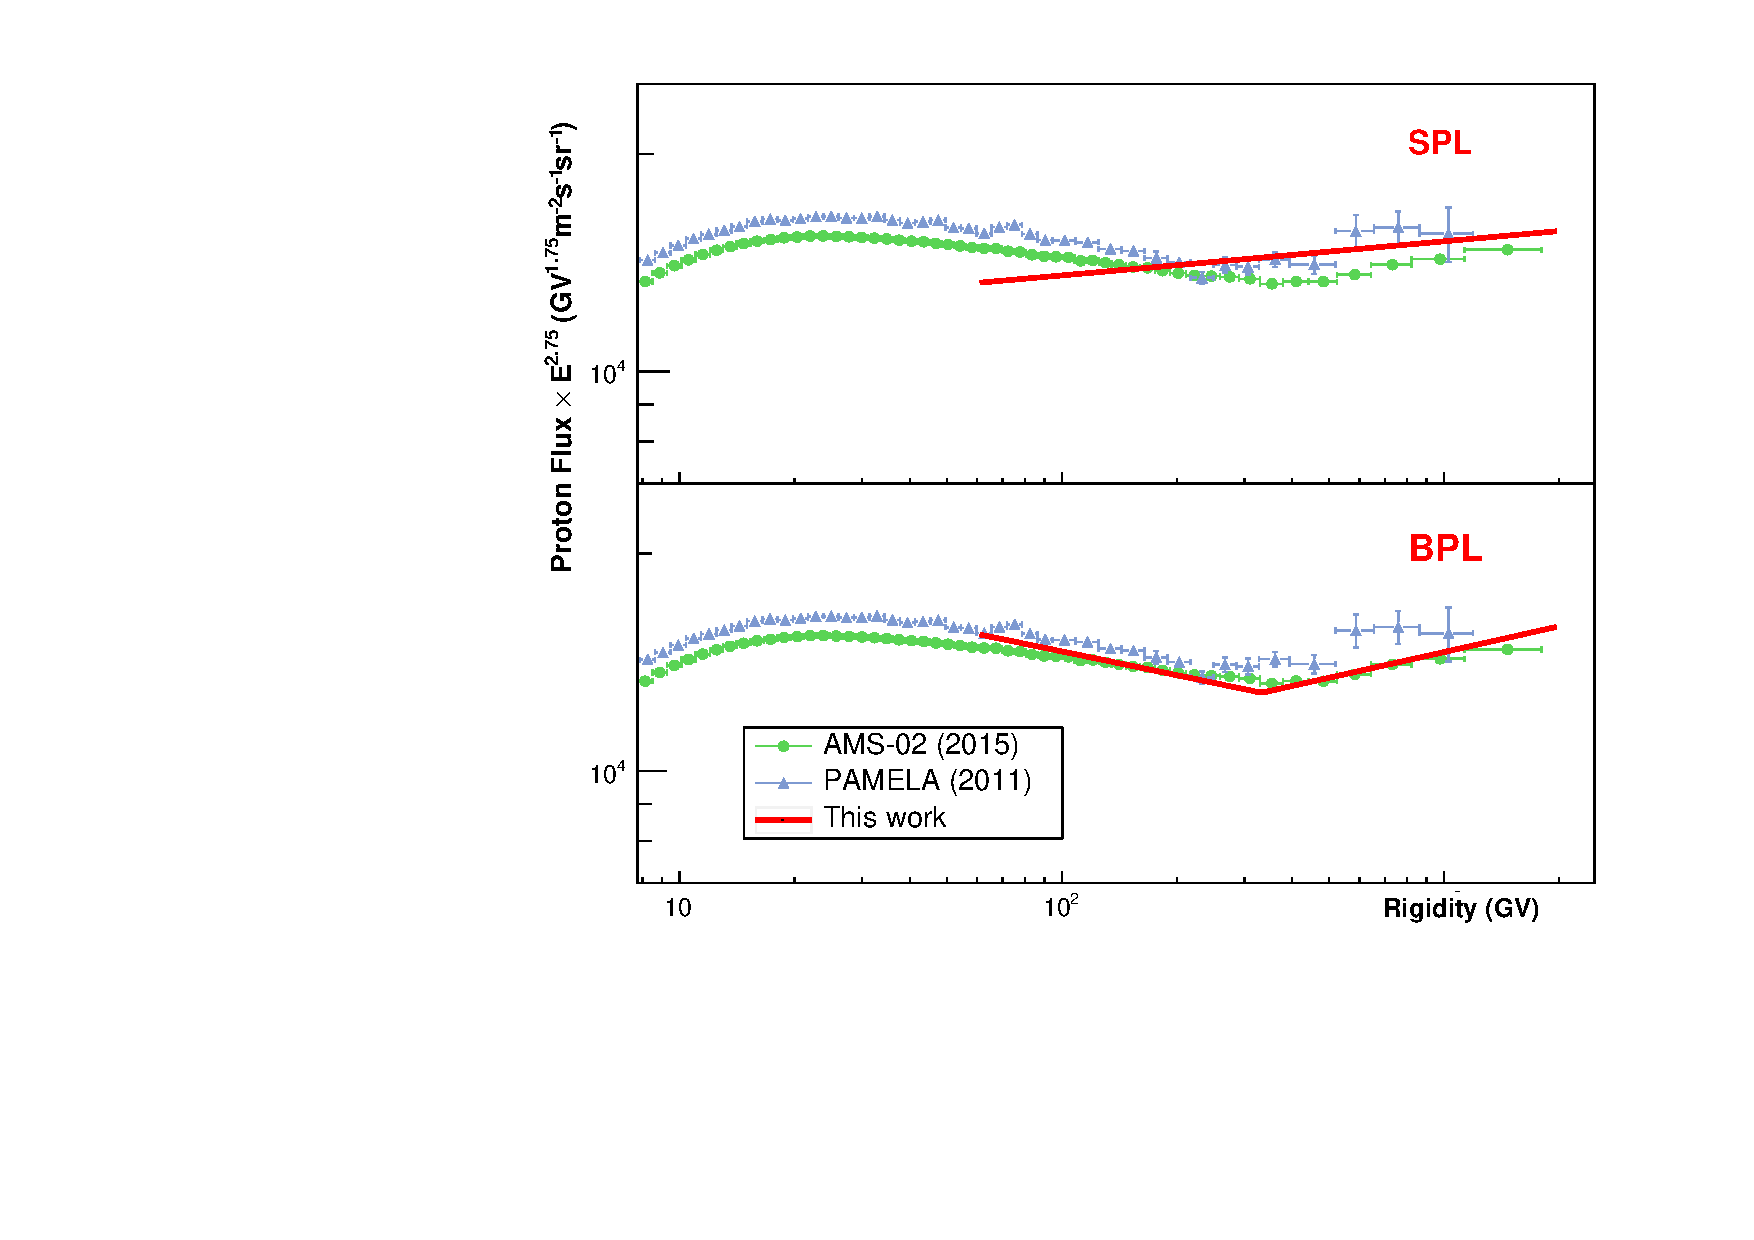
\includegraphics[width=0.9\textwidth]{img/ProtonSpectrumModelMeasurement.pdf}
    % \caption{Best fitted proton CRs versus real observations}
    \caption{Best-fit CR proton spectrum from this work (red) compared to the measurements by AMS-02 (blue) and PAMELA (green).}
    \label{fig:proton-flux}
\end{figure}

% From Figure~\ref{fig:gamma-flux}, a trend of incident proton model
% demonstrated that BPL has more consistency than SPL. Nevertheless,
% to determine the significance between two models require likelihood
% ratio test to evaluate the statistical level of confidence. In addition,
% statistical and total error including the instrument will be determined
% by performing Monte Carlo Simulation.


